% This will be the main document for the Technical Networks paper to
% be written by the Eggnet team of Jordan Ell, Triet Huynh and Braden
% Simpson in association with Adrian Schroeter and Daniela Damian.

\documentclass[conference]{IEEEtran}

% Use of outside images
\usepackage{graphicx} 
% Use text inside euqations
\usepackage{amsmath}

\usepackage{float}
\floatstyle{plaintop}
\restylefloat{table}

% Correct bad hyphenation here
\hyphenation{op-tical net-works semi-conduc-tor}

% Begin the paper here
\begin{document}


% Paper title
% Can use linebreaks \\ within to get better formatting as desired
\title{Kaggle: Adzuna Data Mining Competition}

% Authors names
\author{\IEEEauthorblockN{Jordan Ell}
\IEEEauthorblockA{University of Victoria,
Victoria, British Columbia, Canada \\ jell@uvic.ca}
}

% Make the title area
\maketitle


\begin{abstract}
This paper outlines my attempt to tackle the Kaggle competition entitled ``Job Salary Prediction''
put on by Adzuna. I completed this competition roughly 8 months ago in a team of two. At the time
of completion, I sat 108th in the leader boards. I used a tool created by Yahoo! research called Vowpal
Wabbit, along with many custom python scripts for data manipulation to examine various components
of the training set. I focused largely on free text fields and the keywords that were contained in 
these fields in order to complete this challenge. This challenge has concluded on April 3rd 2013.

\end{abstract}


\section{Introduction}

Data mining can be used to solve many complex problems in modern computing, from determining the most
likely pair of purchases, to recommending movies to users.
Kaggle~\footnote{http://keggle.com}
is a website that is home to many competitions that solve very complex and intriguing problems. It allows companies 
such as Facebook, StackOverflow, and others post data science competitions for cash prizes. The competition that is 
described in this report is job salary prediction, put on by an advertisement search company called 
Adzuna~\footnote{http://adzuna.com}. By predicting the
salary from job posts, Adzuna can provide more accurate ads to their customers. 

The competition is about predicting the 
salary of a job posting based on other attributes in the advertisement. These attributes are described in detail in Section 2, 
and with these attributes I applied algorithms to weigh and train a classifier, from over 240,000 training instances, 
and then tested them on over 40,000 test instances. I used multiple tools and algorithms to obtain a good classifier to this dataset. 
Section 4 will go in detail about the algorithms and the tools used, as well as the motivation for them. The scores obtained are 
measured by the classifier's Mean Absolute Error (MAE), which is then compared to the rest of the world’s submissions to rank them.

The process of the classification was as follows: Data Gathering, Data Preparation, and Data Mining. Gathering consists of 
collecting the data and interpreting their meaning and schema. Preparation is a large step, as the algorithms and tools require 
certain specific types of data and schemas, and getting the raw data to this state can be non-trivial, as in the case of a 
bag-of-words~\footnote{Bag-of-words is a method of processing unstructured text into a dictionary, without grammar, 
punctuation, or language nuances} method of text processing.

I completed this Kaggle challenge roughly 8 months ago with help from Braden Simpson. Upon inspection of date, I sit 268th of 294
(not very well placed but we will see an explanation for this to come).

\section{Data Gathering}

The Adzuna competition was all about trying to predict the salaries of jobs posted
online from a few choice data points. These predictions would help to bring transparency 
to the market while helping potential employees discover the best jobs suited for themselves. 
This being said, the Adzuna team provided all challengers of the Kaggle competition 
with data sets in CSV formats.

There were two main data sets used for this competition. The first set contains the training instances. 
The training instance contains 11 fields of which 10 were attributes with the 11th being the class. 
The 10 attributes were as follows. An ID provides a unique identifier for each job. This ID was 
not used in the actual data mining process but was used to associate jobs to salaries
in the final results of this competition. A title is a free text field that gives the position that an
employer is looking to fill. A full description is a free text field provided by the
job advertisers. This description field holds many of the most interesting potential for future data
mining analysis. This field has been give to the competitors stripped of any text that may directly
refer to salary. The location raw field is a free text field for the location of the job while the
location normalized field is a formal location provided by Adzuna with standard formatting. Contract type
provides a categorical look at full time or part time. Contact time provides a categorical view of
permanent or contract positions. The company field is a free text field for company names. The job category
field is a selection field from 30 standard job categories which employers pick to their needs. Finally, the source
name field provides the email address of the employer. The final column of data is the class which is salary. 
This class is a continuous class and not a categorical or binary class.

The second set of data provided by the Kaggle competition was the validation set
of data. This data again came in the CSV format and again had 11 fields of
which 10 are attributes and 1 as a class. The difference here was that salary has
been stripped from the class field. This file was used as a standard testing file for
all competitor's data models. This was the file of which all tests will be put against.

The size of both of these items of data was quite large. The training CSV file
was over 244,000 records long and the validation data was just over 40,000 records
long. The size of these files needed to be taken into consideration when learning algorithms were applied.

There was also an optional file provided by the Kaggle team called the location
tree. This file was again a CSV file, however, it was used for a different purpose.
This file was used for the purpose of describing the hierarchical nature of the
normalized location field in the training set data. Here the country, direction,
city, and region were all given in order to give sense to the previously mentioned
normalized location data.

For this competition, I simply made use of both the training and validation
sets of data. These pieces of data can be found at the Kaggle
website~\footnote{4http://www.kaggle.com/c/job-salary-prediction/data}.

\section{Data Preperation}

This data mining process intends to use the program Vowpal Wabbit (which
will be explained further in Section 4). Vowpal Wabbit, or VW, takes a custom
input format which needed to be accounted for before any data mining could
take place. While preparing this custom data format, various other steps were
also taken (to be explained) in order to prepare the data for various attempts
and algorithms with data mining. I will outline below the type of input format 
needed, the custom data transformations, as well as data normalization for
future data mining efforts.

The input format for VW is as follows:

\begin{multline}
[Label][Importance[Tag]]|NamespaceFeatures \\ |NamespaceFeatures...|NamespaceFeatures
\end{multline}

where Namespace=String and Features=(String)* or Features=Float. Here we
can see the immediate differences to the original CSV file that are provided
for the Kaggle challenge. The Label is the floating point number that is being
attempted to be predicted. The importance tag can be used to give weight
to a specific training instance over the their instances. This can be useful for
weighted predictions or higher confidence in a particular instance. However,
due to the large number of training instances given for this Kaggle competition
(244,000), the importance tag was not used. Namespace is a value identifier
while features are the values associated with the identifier. In order to transform 
the CSV files to the given VW input format, python scripts were created
and run to make the conversion. While these python scripts were used primarily for 
conversion purposes, they also allowed the tweaking and adjustments of
data as it was converted. I will now explain the different steps taken to tweak
data during the conversion. (The base of the conversion from CSV to VW was
borrowed from FastML5~\footnote{https://github.com/zygmuntz/kaggle-advertised-salaries/blob/master/2vw.py}
while the data tweaks were written from scratch)

As it was shown on the Kaggle website, the data given in the training instanced
represented a skewed bell curve. In order to get this data into a more acceptable
bell curve shape, or normalized (as was needed to VW to run properly, more on
this later), two solutions were used, one at a time. The first was simply to take
the logarithm of the data set. This creates a more acceptable normalization of
the data. That being said, this was the first tweak to be given to the data during
the conversion process. The other available option for creating normalized data
is to take the square root of the instances. This also gave a somewhat more
normalized view of the data. This tweak was also taken on the data although
was preformed at a different time than the logarithm. The results of these two
data tweaks can be seen in Table~\ref{tab:results} as the different types of normalization
transformations.

The second data tweak to be placed on the data during the conversion process
was the limiting of attributes to be used during the training instance model
creation. My python scripts allowed me to adjust which attributes were to be
used for the model generation. Here, I played with one major setting in which
I turned off all free text fields. The results of turning off the free text fields can
again be seen in Table~\ref{tab:results} in relation with the normalization tweaks. A large
number of combinations of free text and categorical attributes could be tested
at any given time with or without keywords with this program. However, due
to the limited time of this competition only the few were actually tested.

The third large tweak to be placed on the data during the conversion process
was the limiting of free text fields to only keywords. In order to make this tweak,
the python library "topia.termextract" was used to extract keywords from local text 
fields. This means that every text field was analyzed separately for
keywords as opposed to looking at all training instances at once. The keyword
threshold for occurrence was set only to 1 as I decided that job descriptions
did not always repeat the most important words at any given rate. This data
tweak was only applied to data for particular runs of the data mining process
and can be seen in the results in Table~\ref{tab:results} for how it was used in relation to
other data tweaks and their outcomes.

The final large tweak to be place on the data during the conversion process
was again involved in limiting the free text fields to only keywords (this was
preformed on separate trials from the aforementioned keywords). The main difference 
here however, was that the global scope of keywords was used instead
of local. This being the case, a python script was created in order to go over
all training instances and extract all keywords used and their frequency of use.
From here a list of the top 500 keywords was then created based on highest
frequencies. Once this list was created, the training instances were converted to
VW as previously mentioned, however, the job description field was limited to
those words that appear in the most frequent keyword list. I did not apply the
keywords to the small free text fields such as location and job title as these free
text fields act much differently than the job descriptions which are much larger
and diverse. The results for these data tweaks can again be seen in Table~\ref{tab:results}.

It should be noted that all of these data tweak were preformed separately except 
for the data normalization. These data tweaks while powerful in their own
right, would not behave nicely when preformed together.

This conversion of data to be handles by a larger data set data mining program
along with the keyword analysis and other data tweaks represent a non trivial
step in this data mining competition.

\section{Data Mining}

For this competition, to reiterate, I attempted to predict job salaries given
some meta information in both categorical and free text forms about the job.
The training set provided by Kaggle to issue this challenge was as astounding
244,000 training instances. This being the case, Weka was not an appropriate
solution to use as a data mining tool as holding this large amount of data in
main memory while preforming standard data mining operations such as SVM
on it would have been devastating in time and space. Another issue with this
size of data were run times, especially when multiple attempts and different data
manipulations were preformed. With these issues present, it was important 
to either write my own algorithms for speed and size, or use a preexisting
tool to handle these scenarios. I went with the latter option.

Solving these issues, I found the data mining tool known as Vowpal Wabbit
(VW). VW is a command line based data mining tool originally created by
Yahoo! Research but was later and more recently sponsored by Microsoft Research. 
VW was designed to be a fast and lightweight tool from the beginning
and accepting of extremely large data sets. VW has a large array of available
data mining algorithms, however, its most prominent algorithm (and algorithm
used for this challenge) is know as the sparse gradient descent (GD) on a loss
function.

The gradient descent algorithm is a similar structure to the type of gradient
descent used in the logistic regression. 
The main difference here is the use of the weight vector in VW’s
gradient descent. The weight vector that VW uses has $2^b$ weights (where b is
the specified by the b option on the command line). What this really means is
that each feature as show in the data preparation section of the VW input, gets
hashed to a particular weight in the vector [0,$2^b$-1] This allows each feature
to have its own particular weight in the gradient descent algorithm. There are
some complex working of what happens when two features get hashed to the
same weight, but I do not feel the need to get into that in the paper as the
feature count was low enough to easily avoid this from happening. (Roughly 
240,000 features in the largest scenarios.) For the loss function of VW,
I decided to use the squared loss function. Given a prediction p and a label
y a loss function measures the discrepancy between the data model’s predicted
outcome and the desired outcome. I selected the squared loss function because 
it has easier input requirements (no real restrictions) than say logistic loss
which requires labels of +1 or -1, as well as squared loss allows for a continuous
prediction model as opposed to binary predictions. The final mention for the
gradient descent method is that input of this method should be normal or close
to. The problem with unnormalized data comes when a step is made in the
gradient descent. At first the (hypothetical) slope of the gradient is so high
that large steps cause an over shooting of the best target value, or the minimum 
of the parabola. Smaller first steps followed by larger later steps can help
the algorithm hone in on the minimum of the parabola easier. Thus having a
bell shape of the input data, or having it normalized, gives a better process
towards finding the minimum of the parabola.

VW comes with its own unique input format as was described in the data
preparation section of this paper. However what was not fully explained was
the flexibility of the input and how the input’s features are interpreted in the
data mining process. (Refer to Equation 1 for the following explanation.) The
label is the most important feature of the input, which is the class attribute of
the training instance. Since VW is expecting a normalized input in terms of
the distribution of class values in the training instance, it is important for this
tool that the training instance be normalized with either the logarithm function
or the square root function before running. More importantly, is the way that
VW handles free text fields as described in the previous section. VW uses
something called a Bag-of-Words model in order to interpret free text fields. An
explanation of free text fields can be seen in Figure~\ref{fig:bag}.

\begin{figure*}[tb!]
\centering
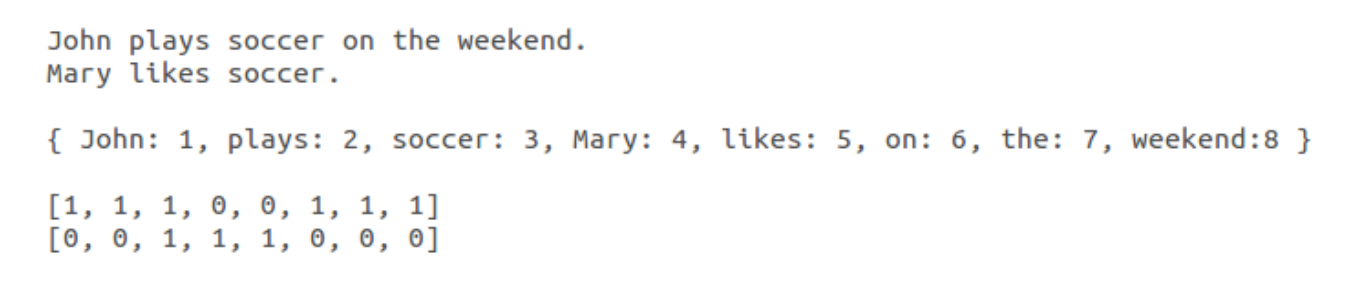
\includegraphics[width=0.9\textwidth]{images/bag.png}
\caption{A bag of words placed into a vector\label{fig:bag}}
\end{figure*}

Some things to notes about this example. The dictionary constructed in the
second step does not have to appear in the same order that the words are found
in the text. After extraction, each word is represented by a 8-entry vector. The
terms in the vector are then subject to weighting. The weighting is preformed
by the gradient descent algorithm that was described above and the weights in
the large b-weight vector as previously described. This way of data mining free
text fields is very common among data mining applications.

For the actual data mining process, 6 main data trials were given as input to
the VW program. These trials and their data varied as follows. First, a simplistic 
approach was taken by excluding all bag of words columns in the training
instances. Bag of words form the most complex data mining rules and therefore
are excluded to create a base line analysis of where the tool will finish without
any of the added complexity. This data set trial was used with both the logarithmic 
first and square root functions of data normalization. (All data trials
from now on are used once with logarithmic and once with square root normalization.) 
These results of these base line trials runs can be found in Table~\ref{tab:results}
in the last section of the paper. The next trial run on the data mining
algorithm (gradient descent) was called the full bag of words run. Here,
all columns that are bag of words and not categorical were used in addition to
all categorical columns. The main note here is that the bag of words columns
were preprocessed in order to eliminate numbers, abbreviations, or any other
text that cannot be classified in a standard dictionary. This preprocessing only
leaves English words in the free text columns of the training instances. The
results of this trial run can again be found in Table~\ref{tab:results}. The final, and most
complex trial run against the gradient descent algorithm was called
bag of keywords. As the title of this trial gives away, I was only concerned
with keywords in the free text columns of the training instances. In order to get
the keywords of a particular bag of text, the python library known as 
Topia~\footnote{6https://pypi.python.org/pypi/topia.termextract/}
was used. Topia is a natural language processor library which can (with some
flexibility) extract the keywords from a block of text. An example of keywords
are as follows. The text "The fox can’t jump over the fox’s tail." in Topia yields
the results: [(’tail’, 1, 1), (’fox’, 2, 1)]. As it can easily be seen, the keywords
of tail and fox have been extracted from the main body of text as keywords.
What is less obvious are the remaining digits provided by Topia. This is
where the flexibility of Topia comes into play. In each triple, the keyword, the
occurrences, and the number of words in the keyword are given. This being the
case, I was able to set thresholds on Topia’s extractions in order to limit the
keywords selected. We can limit the keywords to only those repeated in the
text body at least once, or those that are composed of at least two words and
so on. However, for simplicity of the main data trials, I allowed Topia the
lowest of thresholds for keyword extraction, being no repeat and single words.
This allowed me to again create a base line measurement of keyword usage in the
data mining process. Again preprocessing was done on the training instances
in order to limit the free text columns to key words only. The results of this
baseline keyword run in VW can be seen in Table~\ref{tab:results}.

Aside from the 6 main trials, 2 additional trials (with square root and log) were
given as the global keyword system described in the Data Preparation section of
this paper. This was the final ditch effort used in data mining for this competition.
Once the global keywords had been collected by the python script, the CSV to
VW script was slightly modified in order to only include the words in the full
description of the job which appeared in the global keyword list. For simplicity,
the global keywords list was limited to 500 words as it was felt that these keywords
should yield better results compared to a larger list.

\section{Results and Conclusions}

This section contains the main results table for the 6 main data trial runs as
described in the data mining section of this paper. All results are expressed in
mean absolute error (MAE). The MAE is calculated when uploading potential
results to the Kaggle website competition. The MAE is exactly what is sounds
like, in that it is the average "dollars off" between my estimate created using
the data mining model and the actual answer known only by Kaggle.

\begin{table}[h]
\begin{center}
\begin{tabular}{| c | c | c |}
\hline
Free Text & Logarithmic & Square Root \\
\hline
\hline
None & 12712.17 & 13293.12 \\ \hline
All & 7350.44 & 7175.04 \\ \hline
Keywords (local) & 8149.91 & 7744.84 \\ \hline
Keywords (global) & 8360.31544 & 8135.83 \\ \hline
\end{tabular}
\end{center}
\caption{Results from main data trial runs.\label{tab:results}}
\end{table}

As can be seen in the table above, the baseline scenario of no bag of words used
in the data mining process yielded by far the worst results. This was largely
expected based on the nature of the Kaggle competition. If data mining was
better without bag of word usage, these types of challenges may not be ever
needed as the simplicity of data mining would be trivial. Where the power and
knowledge of this competition really came from was the use of the bag of words or
free text columns in the training instances and how they could be used to better
the results of any data mining predictions.

The next main data trial run was that on the full bag of words or free text
columns inside the VW data mining tool. These results were vastly superior to
those of the non free text trials. This was also largely to be expected. Some
notes to take away from these results were as follows. For one, the use of all
words in free text columns and the VW data mining tools using the gradient
descent algorithm scored a lower MAE than the benchmark set by Kaggle (at the time) which
was a random forest algorithm. The Kaggle benchmark with the random forest
was 7536.29 which was beat by the full bag of words run I preformed. This
already was showing promise for the use of the VW tool over a standard tool such
as Weka which may just be able to load the data and preform analysis. The
Kaggle random forest benchmark was also said to take 1.5 hours on a 2.7GHz
processor the 8 cores and 8GB of RAM. The VW tool took around 5 minutes to
fully complete its run cycle. The last thing to note from this full bag of words
trial was that it put me into 108th spot on the Kaggle leader-boards (at the time) for this
challenge out of 253 participating teams. This was a large success for this project.

The final result for the main data trial sets was that of the keywords (local) from
the keyword selection of the bag of words columns in the training instances. I was
surprised that the keywords did not help create a better solution than just
a full bag of words. If anything the local keywords should have helped alleviate
pressure from words such as "the", "it", "and" and so on. The issue may lie in
the fact that using keywords will break up key sentences that are more telling
than keywords. Perhaps this would be worth exploring in the future.

As part of the last ditch effort of keywords, the global keyword trials can be
seen in the keywords (global) row. These results were actually slightly worse
than local keywords. A reminder, the difference between global and local was
that global keywords were examined over the entire training instances and then
limited to the top 500 keywords based on occurrence. Again the limiting of
words would seem like a better idea than using all words in the free text fields,
however, these limitations use less vector weights which could ultimately be the
reason for the worse final results.

In conclusion, I experimented with various trial runs of gradient descent in
VW with different data parsing on free text fields. I eventually discovered
that the linear gradient descent algorithm works better with a larger collection
of words for a higher number of weight vectors. I have presented various way
in which keywords can be extracted from CSV files and used for data mining
practices. I have also drawn the conclusion that bag of words algorithms
prefer larger bag of words compared to smaller more refined set of words.

% End of the paper
\end{document}
